\section{Competition Outlines}

\subsection{Playing Field}

The playing field is a rectangular area with the following dimensions:

\begin{itemize}
	\item Length: 36 meters
	\item Width: 18 meters
	\item Height: 6 meters
\end{itemize}


The playing field is divided into three zones:
\begin{itemize}
	\item \textbf{Two Team Zones (red and blue):} The home base of each team, where the drones start and land.
	\item \textbf{One Neutral Zone in the middle:} A neutral territory for strategic maneuvers.
\end{itemize}

The field layout is illustrated in the figure below:

\begin{figure}[H]
\centering


\tikzset{every picture/.style={line width=0.75pt}} %set default line width to 0.75pt        

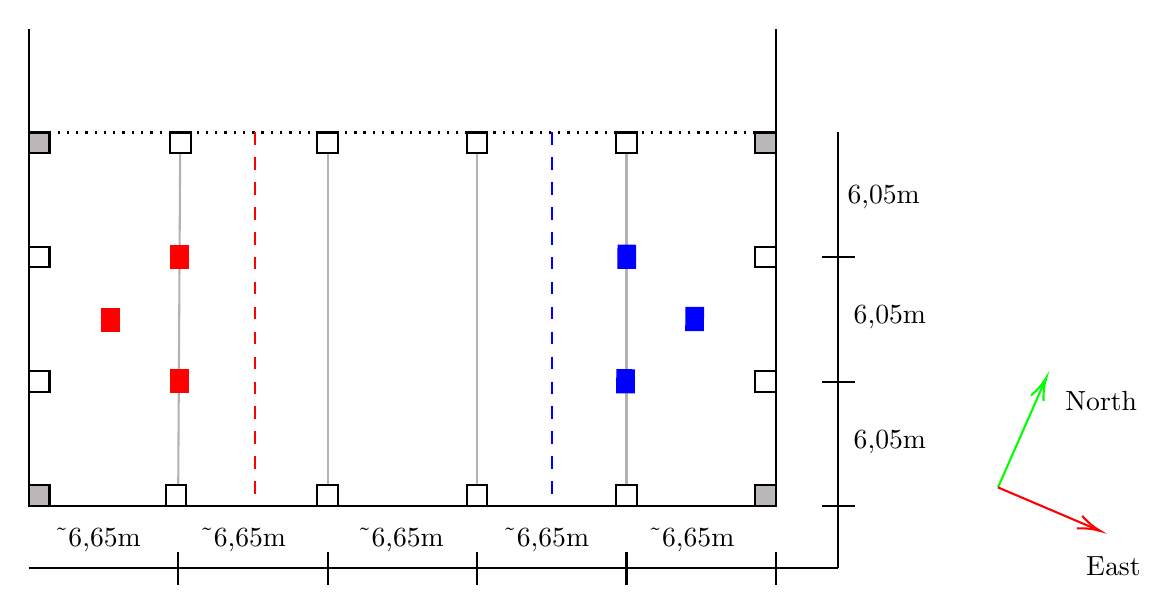
\begin{tikzpicture}[x=0.75pt,y=0.75pt,yscale=-1,xscale=1]
%uncomment if require: \path (0,300); %set diagram left start at 0, and has height of 300

%Straight Lines [id:da732117601547551] 
\draw [color={rgb, 255:red, 178; green, 178; blue, 178 }  ,draw opacity=1 ]   (368,62.7) -- (368,240) ;
%Straight Lines [id:da11547189962690729] 
\draw [color={rgb, 255:red, 178; green, 178; blue, 178 }  ,draw opacity=1 ]   (296,62.7) -- (296,240) ;
%Shape: Rectangle [id:dp5257365870856812] 
\draw  [fill={rgb, 255:red, 188; green, 183; blue, 183 }  ,fill opacity=1 ] (80,230) -- (90,230) -- (90,240) -- (80,240) -- cycle ;
%Shape: Rectangle [id:dp6902751554964373] 
\draw  [fill={rgb, 255:red, 188; green, 183; blue, 183 }  ,fill opacity=1 ] (80,60) -- (90,60) -- (90,70) -- (80,70) -- cycle ;
%Shape: Rectangle [id:dp7175934918184133] 
\draw   (80,115) -- (90,115) -- (90,125) -- (80,125) -- cycle ;
%Shape: Rectangle [id:dp6947267906952321] 
\draw   (80,175) -- (90,175) -- (90,185) -- (80,185) -- cycle ;
%Shape: Rectangle [id:dp18912389410211783] 
\draw  [fill={rgb, 255:red, 188; green, 183; blue, 183 }  ,fill opacity=1 ] (430,230) -- (440,230) -- (440,240) -- (430,240) -- cycle ;
%Shape: Rectangle [id:dp9930645821346726] 
\draw  [fill={rgb, 255:red, 188; green, 183; blue, 183 }  ,fill opacity=1 ] (430,60) -- (440,60) -- (440,70) -- (430,70) -- cycle ;
%Shape: Rectangle [id:dp12124178621662995] 
\draw   (430,115) -- (440,115) -- (440,125) -- (430,125) -- cycle ;
%Shape: Rectangle [id:dp9831498985278126] 
\draw   (430,175) -- (440,175) -- (440,185) -- (430,185) -- cycle ;
%Straight Lines [id:da05129566016673692] 
\draw [color={rgb, 255:red, 178; green, 178; blue, 178 }  ,draw opacity=1 ]   (153,64.1) -- (152,236.63) ;
%Shape: Rectangle [id:dp4499234743016205] 
\draw  [fill={rgb, 255:red, 255; green, 255; blue, 255 }  ,fill opacity=1 ] (146,230) -- (156,230) -- (156,240) -- (146,240) -- cycle ;
%Shape: Rectangle [id:dp7847482817794953] 
\draw  [fill={rgb, 255:red, 255; green, 255; blue, 255 }  ,fill opacity=1 ] (148,60) -- (158,60) -- (158,70) -- (148,70) -- cycle ;
%Shape: Rectangle [id:dp9580154784702117] 
\draw  [fill={rgb, 255:red, 255; green, 255; blue, 255 }  ,fill opacity=1 ] (363,230) -- (373,230) -- (373,240) -- (363,240) -- cycle ;
%Shape: Rectangle [id:dp9344209704588882] 
\draw  [draw opacity=0][fill={rgb, 255:red, 255; green, 0; blue, 0 }  ,fill opacity=1 ] (148,174) -- (157,174) -- (157,185.67) -- (148,185.67) -- cycle ;
%Straight Lines [id:da24551702903482164] 
\draw    (80,10) -- (80,230) ;
%Straight Lines [id:da859606388896009] 
\draw    (430,240) -- (90,240) ;
%Straight Lines [id:da3323697707442079] 
\draw    (440,230) -- (440,10) ;
%Straight Lines [id:da4136030529491721] 
\draw  [dash pattern={on 0.84pt off 2.51pt}]  (430,60) -- (90,60) ;
%Straight Lines [id:da5164909031289946] 
\draw [color={rgb, 255:red, 178; green, 178; blue, 178 }  ,draw opacity=1 ]   (224,59.33) -- (224,236.63) ;
%Shape: Rectangle [id:dp3648375872831182] 
\draw  [fill={rgb, 255:red, 255; green, 255; blue, 255 }  ,fill opacity=1 ] (219,230) -- (229,230) -- (229,240) -- (219,240) -- cycle ;
%Shape: Rectangle [id:dp0407090254865925] 
\draw  [fill={rgb, 255:red, 255; green, 255; blue, 255 }  ,fill opacity=1 ] (291,230) -- (301,230) -- (301,240) -- (291,240) -- cycle ;
%Shape: Rectangle [id:dp3730561773093124] 
\draw  [fill={rgb, 255:red, 255; green, 255; blue, 255 }  ,fill opacity=1 ] (219,60) -- (229,60) -- (229,70) -- (219,70) -- cycle ;
%Straight Lines [id:da29809430805096926] 
\draw    (80,270) -- (470,270) (152,262) -- (152,278)(224,262) -- (224,278)(296,262) -- (296,278)(368,262) -- (368,278)(440,262) -- (440,278) ;
%Straight Lines [id:da5550576509758283] 
\draw    (470,60) -- (470,270) (478,120) -- (462,120)(478,180) -- (462,180)(478,240) -- (462,240) ;
%Shape: Rectangle [id:dp21734988290391533] 
\draw  [draw opacity=0][fill={rgb, 255:red, 255; green, 0; blue, 0 }  ,fill opacity=1 ] (148,114) -- (157,114) -- (157,125.67) -- (148,125.67) -- cycle ;
%Shape: Rectangle [id:dp3252282288402786] 
\draw  [draw opacity=0][fill={rgb, 255:red, 255; green, 0; blue, 0 }  ,fill opacity=1 ] (115,144.33) -- (124,144.33) -- (124,156) -- (115,156) -- cycle ;
%Shape: Rectangle [id:dp0188017080720857] 
\draw  [draw opacity=0][fill={rgb, 255:red, 0; green, 0; blue, 255 }  ,fill opacity=1 ] (372.58,125.75) -- (363.58,125.67) -- (363.69,114) -- (372.69,114.09) -- cycle ;
%Shape: Rectangle [id:dp5993605107726458] 
\draw  [draw opacity=0][fill={rgb, 255:red, 0; green, 0; blue, 255 }  ,fill opacity=1 ] (372,185.75) -- (363,185.66) -- (363.11,174) -- (372.11,174.08) -- cycle ;
%Shape: Rectangle [id:dp3269940382054979] 
\draw  [draw opacity=0][fill={rgb, 255:red, 0; green, 0; blue, 255 }  ,fill opacity=1 ] (405.29,155.73) -- (396.29,155.65) -- (396.4,143.98) -- (405.4,144.07) -- cycle ;
%Shape: Rectangle [id:dp32798188101744863] 
\draw  [fill={rgb, 255:red, 255; green, 255; blue, 255 }  ,fill opacity=1 ] (363,60) -- (373,60) -- (373,70) -- (363,70) -- cycle ;
%Shape: Rectangle [id:dp40180864334923094] 
\draw  [fill={rgb, 255:red, 255; green, 255; blue, 255 }  ,fill opacity=1 ] (291,60) -- (301,60) -- (301,70) -- (291,70) -- cycle ;
%Straight Lines [id:da3874188576128408] 
\draw [color={rgb, 255:red, 255; green, 0; blue, 0 }  ,draw opacity=1 ] [dash pattern={on 4.5pt off 4.5pt}]  (189,60) -- (189,240) ;
%Straight Lines [id:da8233851227369617] 
\draw [color={rgb, 255:red, 0; green, 0; blue, 255 }  ,draw opacity=1 ] [dash pattern={on 4.5pt off 4.5pt}]  (332,60) -- (332,240) ;
%Straight Lines [id:da4588832698718919] 
\draw [color={rgb, 255:red, 0; green, 255; blue, 0 }  ,draw opacity=1 ]   (547,231) -- (569.53,179.83) ;
\draw [shift={(570.33,178)}, rotate = 113.76] [color={rgb, 255:red, 0; green, 255; blue, 0 }  ,draw opacity=1 ][line width=0.75]    (10.93,-3.29) .. controls (6.95,-1.4) and (3.31,-0.3) .. (0,0) .. controls (3.31,0.3) and (6.95,1.4) .. (10.93,3.29)   ;
%Straight Lines [id:da4775954924120087] 
\draw [color={rgb, 255:red, 255; green, 0; blue, 0 }  ,draw opacity=1 ]   (547,231) -- (594.49,251.22) ;
\draw [shift={(596.33,252)}, rotate = 203.06] [color={rgb, 255:red, 255; green, 0; blue, 0 }  ,draw opacity=1 ][line width=0.75]    (10.93,-3.29) .. controls (6.95,-1.4) and (3.31,-0.3) .. (0,0) .. controls (3.31,0.3) and (6.95,1.4) .. (10.93,3.29)   ;

% Text Node
\draw (91,249) node [anchor=north west][inner sep=0.75pt]   [align=left] {\textasciitilde 6,65m};
% Text Node
\draw (476,202) node [anchor=north west][inner sep=0.75pt]   [align=left] {6,05m};
% Text Node
\draw (161,249) node [anchor=north west][inner sep=0.75pt]   [align=left] {\textasciitilde 6,65m};
% Text Node
\draw (237,249) node [anchor=north west][inner sep=0.75pt]   [align=left] {\textasciitilde 6,65m};
% Text Node
\draw (307,249) node [anchor=north west][inner sep=0.75pt]   [align=left] {\textasciitilde 6,65m};
% Text Node
\draw (377,249) node [anchor=north west][inner sep=0.75pt]   [align=left] {\textasciitilde 6,65m};
% Text Node
\draw (476,142) node [anchor=north west][inner sep=0.75pt]   [align=left] {6,05m};
% Text Node
\draw (473,84) node [anchor=north west][inner sep=0.75pt]   [align=left] {6,05m};
% Text Node
\draw (578,183) node [anchor=north west][inner sep=0.75pt]   [align=left] {North};
% Text Node
\draw (588,263) node [anchor=north west][inner sep=0.75pt]   [align=left] {East};


\end{tikzpicture}

\caption{Field Dimensions}
\end{figure}

The sizes shown in the graphic are approximate values. The exact dimensions may vary slightly.

\subsection{Indoor Positioning System}

The challenge will take place in a hangar at the Manching Airport (48°43'21.7"N 11°33'04.9"E).
To imporve the state estimation in a potential gps denied environment, a camera based positioning system using ArUco marker can be used.
Two ArUco marker are attached to each pillar in the hangar.
The figure below illustrates the IDs of the maker that are attached to the pillars, where the lower ArUco marker is mounted at a height of 2m and the upper marker at 4m.

\begin{figure}[H]

\centering

\tikzset{every picture/.style={line width=0.75pt}} %set default line width to 0.75pt        

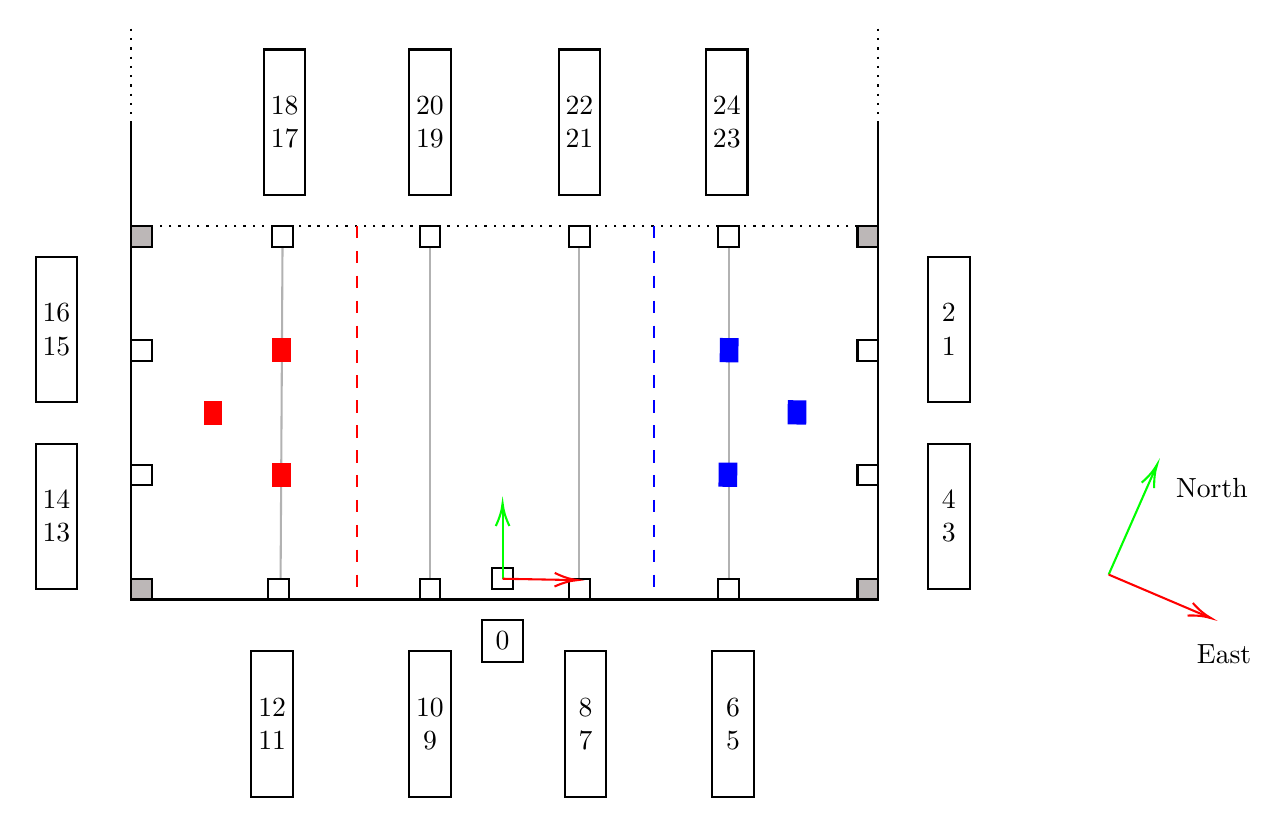
\begin{tikzpicture}[x=0.75pt,y=0.75pt,yscale=-1,xscale=1]
%uncomment if require: \path (0,403); %set diagram left start at 0, and has height of 403

%Straight Lines [id:da8324081494103803] 
\draw [color={rgb, 255:red, 178; green, 178; blue, 178 }  ,draw opacity=1 ]   (344,97.7) -- (344,275) ;
%Straight Lines [id:da9583452157235313] 
\draw [color={rgb, 255:red, 178; green, 178; blue, 178 }  ,draw opacity=1 ]   (272,97.7) -- (272,275) ;
%Shape: Rectangle [id:dp3433626255284923] 
\draw  [fill={rgb, 255:red, 188; green, 183; blue, 183 }  ,fill opacity=1 ] (56,265) -- (66,265) -- (66,275) -- (56,275) -- cycle ;
%Shape: Rectangle [id:dp6616954858549284] 
\draw  [fill={rgb, 255:red, 188; green, 183; blue, 183 }  ,fill opacity=1 ] (56,95) -- (66,95) -- (66,105) -- (56,105) -- cycle ;
%Shape: Rectangle [id:dp2948289764970793] 
\draw   (56,150) -- (66,150) -- (66,160) -- (56,160) -- cycle ;
%Shape: Rectangle [id:dp6971973555173374] 
\draw   (56,210) -- (66,210) -- (66,220) -- (56,220) -- cycle ;
%Shape: Rectangle [id:dp9126690703683185] 
\draw  [fill={rgb, 255:red, 188; green, 183; blue, 183 }  ,fill opacity=1 ] (406,265) -- (416,265) -- (416,275) -- (406,275) -- cycle ;
%Shape: Rectangle [id:dp36362493354229275] 
\draw  [fill={rgb, 255:red, 188; green, 183; blue, 183 }  ,fill opacity=1 ] (406,95) -- (416,95) -- (416,105) -- (406,105) -- cycle ;
%Shape: Rectangle [id:dp7438280632958825] 
\draw   (406,150) -- (416,150) -- (416,160) -- (406,160) -- cycle ;
%Shape: Rectangle [id:dp8190129040006575] 
\draw   (406,210) -- (416,210) -- (416,220) -- (406,220) -- cycle ;
%Straight Lines [id:da6821139759238273] 
\draw [color={rgb, 255:red, 178; green, 178; blue, 178 }  ,draw opacity=1 ]   (129,99.1) -- (128,271.63) ;
%Shape: Rectangle [id:dp12978164760841726] 
\draw  [fill={rgb, 255:red, 255; green, 255; blue, 255 }  ,fill opacity=1 ] (122,265) -- (132,265) -- (132,275) -- (122,275) -- cycle ;
%Shape: Rectangle [id:dp7976816015193462] 
\draw  [fill={rgb, 255:red, 255; green, 255; blue, 255 }  ,fill opacity=1 ] (124,95) -- (134,95) -- (134,105) -- (124,105) -- cycle ;
%Shape: Rectangle [id:dp9966657246268984] 
\draw  [fill={rgb, 255:red, 255; green, 255; blue, 255 }  ,fill opacity=1 ] (339,265) -- (349,265) -- (349,275) -- (339,275) -- cycle ;
%Shape: Rectangle [id:dp5757119210618549] 
\draw  [draw opacity=0][fill={rgb, 255:red, 255; green, 0; blue, 0 }  ,fill opacity=1 ] (124,209) -- (133,209) -- (133,220.67) -- (124,220.67) -- cycle ;
%Straight Lines [id:da32211068188423364] 
\draw    (56,45) -- (56,265) ;
%Straight Lines [id:da4667069569376905] 
\draw    (406,275) -- (66,275) ;
%Straight Lines [id:da936931704558561] 
\draw    (416,265) -- (416,45) ;
%Straight Lines [id:da9729387023000151] 
\draw  [dash pattern={on 0.84pt off 2.51pt}]  (406,95) -- (66,95) ;
%Straight Lines [id:da5555743691262991] 
\draw [color={rgb, 255:red, 178; green, 178; blue, 178 }  ,draw opacity=1 ]   (200,94.33) -- (200,271.63) ;
%Shape: Rectangle [id:dp7316698787727904] 
\draw  [fill={rgb, 255:red, 255; green, 255; blue, 255 }  ,fill opacity=1 ] (195,265) -- (205,265) -- (205,275) -- (195,275) -- cycle ;
%Shape: Rectangle [id:dp5859859750919403] 
\draw  [fill={rgb, 255:red, 255; green, 255; blue, 255 }  ,fill opacity=1 ] (267,265) -- (277,265) -- (277,275) -- (267,275) -- cycle ;
%Shape: Rectangle [id:dp1572370552698623] 
\draw  [fill={rgb, 255:red, 255; green, 255; blue, 255 }  ,fill opacity=1 ] (195,95) -- (205,95) -- (205,105) -- (195,105) -- cycle ;
%Shape: Rectangle [id:dp9841641512210579] 
\draw  [draw opacity=0][fill={rgb, 255:red, 255; green, 0; blue, 0 }  ,fill opacity=1 ] (124,149) -- (133,149) -- (133,160.67) -- (124,160.67) -- cycle ;
%Shape: Rectangle [id:dp039623004192071765] 
\draw  [draw opacity=0][fill={rgb, 255:red, 255; green, 0; blue, 0 }  ,fill opacity=1 ] (91,179.33) -- (100,179.33) -- (100,191) -- (91,191) -- cycle ;
%Shape: Rectangle [id:dp5350102750244554] 
\draw  [draw opacity=0][fill={rgb, 255:red, 0; green, 0; blue, 255 }  ,fill opacity=1 ] (348.58,160.75) -- (339.58,160.67) -- (339.69,149) -- (348.69,149.09) -- cycle ;
%Shape: Rectangle [id:dp8150990393346593] 
\draw  [draw opacity=0][fill={rgb, 255:red, 0; green, 0; blue, 255 }  ,fill opacity=1 ] (348,220.75) -- (339,220.66) -- (339.11,209) -- (348.11,209.08) -- cycle ;
%Shape: Rectangle [id:dp37866285102082187] 
\draw  [draw opacity=0][fill={rgb, 255:red, 0; green, 0; blue, 255 }  ,fill opacity=1 ] (381.29,190.73) -- (372.29,190.65) -- (372.4,178.98) -- (381.4,179.07) -- cycle ;
%Shape: Rectangle [id:dp3600599674807883] 
\draw  [fill={rgb, 255:red, 255; green, 255; blue, 255 }  ,fill opacity=1 ] (339,95) -- (349,95) -- (349,105) -- (339,105) -- cycle ;
%Shape: Rectangle [id:dp4499187841739831] 
\draw  [fill={rgb, 255:red, 255; green, 255; blue, 255 }  ,fill opacity=1 ] (267,95) -- (277,95) -- (277,105) -- (267,105) -- cycle ;
%Straight Lines [id:da4108053166014911] 
\draw [color={rgb, 255:red, 0; green, 255; blue, 0 }  ,draw opacity=1 ]   (527,263) -- (549.53,211.83) ;
\draw [shift={(550.33,210)}, rotate = 113.76] [color={rgb, 255:red, 0; green, 255; blue, 0 }  ,draw opacity=1 ][line width=0.75]    (10.93,-3.29) .. controls (6.95,-1.4) and (3.31,-0.3) .. (0,0) .. controls (3.31,0.3) and (6.95,1.4) .. (10.93,3.29)   ;
%Straight Lines [id:da8518368663842253] 
\draw [color={rgb, 255:red, 255; green, 0; blue, 0 }  ,draw opacity=1 ]   (527,263) -- (574.49,283.22) ;
\draw [shift={(576.33,284)}, rotate = 203.06] [color={rgb, 255:red, 255; green, 0; blue, 0 }  ,draw opacity=1 ][line width=0.75]    (10.93,-3.29) .. controls (6.95,-1.4) and (3.31,-0.3) .. (0,0) .. controls (3.31,0.3) and (6.95,1.4) .. (10.93,3.29)   ;
%Shape: Rectangle [id:dp47541913233873645] 
\draw  [fill={rgb, 255:red, 255; green, 255; blue, 255 }  ,fill opacity=1 ] (230,260) -- (240,260) -- (240,270) -- (230,270) -- cycle ;
%Shape: Rectangle [id:dp7925913677020975] 
\draw   (440,110) -- (460,110) -- (460,180) -- (440,180) -- cycle ;
%Shape: Rectangle [id:dp5853821618437607] 
\draw   (440,200) -- (460,200) -- (460,270) -- (440,270) -- cycle ;
%Shape: Rectangle [id:dp8950595692026859] 
\draw   (336,300) -- (356,300) -- (356,370) -- (336,370) -- cycle ;
%Shape: Rectangle [id:dp8736581379567236] 
\draw   (265,300) -- (285,300) -- (285,370) -- (265,370) -- cycle ;
%Shape: Rectangle [id:dp7016375790720544] 
\draw   (190,300) -- (210,300) -- (210,370) -- (190,370) -- cycle ;
%Shape: Rectangle [id:dp6651707993087799] 
\draw   (114,300) -- (134,300) -- (134,370) -- (114,370) -- cycle ;
%Shape: Rectangle [id:dp28408371720304637] 
\draw   (10,200) -- (30,200) -- (30,270) -- (10,270) -- cycle ;
%Shape: Rectangle [id:dp18377599545402856] 
\draw   (10,110) -- (30,110) -- (30,180) -- (10,180) -- cycle ;
%Shape: Rectangle [id:dp4541157924861472] 
\draw   (120,10) -- (140,10) -- (140,80) -- (120,80) -- cycle ;
%Shape: Rectangle [id:dp6243825023601357] 
\draw   (190,10) -- (210,10) -- (210,80) -- (190,80) -- cycle ;
%Shape: Rectangle [id:dp32078336968864973] 
\draw   (262,10) -- (282,10) -- (282,80) -- (262,80) -- cycle ;
%Shape: Rectangle [id:dp260406599862427] 
\draw   (333,10) -- (353,10) -- (353,80) -- (333,80) -- cycle ;
%Straight Lines [id:da11335481038338502] 
\draw [color={rgb, 255:red, 0; green, 255; blue, 0 }  ,draw opacity=1 ]   (235,265) -- (235,230.67) ;
\draw [shift={(235,228.67)}, rotate = 90] [color={rgb, 255:red, 0; green, 255; blue, 0 }  ,draw opacity=1 ][line width=0.75]    (10.93,-3.29) .. controls (6.95,-1.4) and (3.31,-0.3) .. (0,0) .. controls (3.31,0.3) and (6.95,1.4) .. (10.93,3.29)   ;
%Straight Lines [id:da5821141127690854] 
\draw [color={rgb, 255:red, 255; green, 0; blue, 0 }  ,draw opacity=1 ]   (235,265) -- (269,265.63) ;
\draw [shift={(271,265.67)}, rotate = 181.06] [color={rgb, 255:red, 255; green, 0; blue, 0 }  ,draw opacity=1 ][line width=0.75]    (10.93,-3.29) .. controls (6.95,-1.4) and (3.31,-0.3) .. (0,0) .. controls (3.31,0.3) and (6.95,1.4) .. (10.93,3.29)   ;
%Shape: Rectangle [id:dp33729774098233656] 
\draw   (225,285) -- (245,285) -- (245,305) -- (225,305) -- cycle ;
%Straight Lines [id:da8915486331517322] 
\draw  [dash pattern={on 0.84pt off 2.51pt}]  (56,0) -- (56,220) ;
%Straight Lines [id:da4635661102038766] 
\draw  [dash pattern={on 0.84pt off 2.51pt}]  (416,0) -- (416,220) ;
%Straight Lines [id:da23401687089544798] 
\draw [color={rgb, 255:red, 255; green, 0; blue, 0 }  ,draw opacity=1 ] [dash pattern={on 4.5pt off 4.5pt}]  (165,95) -- (165,275) ;
%Straight Lines [id:da6738294185264133] 
\draw [color={rgb, 255:red, 0; green, 0; blue, 255 }  ,draw opacity=1 ] [dash pattern={on 4.5pt off 4.5pt}]  (308,95) -- (308,275) ;

% Text Node
\draw (558,215) node [anchor=north west][inner sep=0.75pt]   [align=left] {North};
% Text Node
\draw (568,295) node [anchor=north west][inner sep=0.75pt]   [align=left] {East};
% Text Node
\draw (450,145) node   [align=left] {2\\1};
% Text Node
\draw (450,235) node   [align=left] {4\\3};
% Text Node
\draw (346,335) node   [align=left] {6\\5};
% Text Node
\draw (275,335) node   [align=left] {8\\7};
% Text Node
\draw (200,335) node   [align=left] {\begin{minipage}[lt]{14.06pt}\setlength\topsep{0pt}
\begin{center}
10\\9
\end{center}

\end{minipage}};
% Text Node
\draw (124,335) node   [align=left] {\begin{minipage}[lt]{14.06pt}\setlength\topsep{0pt}
\begin{center}
12\\11
\end{center}

\end{minipage}};
% Text Node
\draw (20,235) node   [align=left] {\begin{minipage}[lt]{14.06pt}\setlength\topsep{0pt}
\begin{center}
14\\13
\end{center}

\end{minipage}};
% Text Node
\draw (20,145) node   [align=left] {16\\15};
% Text Node
\draw (130,45) node   [align=left] {\begin{minipage}[lt]{14.06pt}\setlength\topsep{0pt}
\begin{center}
18\\17
\end{center}

\end{minipage}};
% Text Node
\draw (200,45) node   [align=left] {20\\19};
% Text Node
\draw (272,45) node   [align=left] {22\\21};
% Text Node
\draw (343,45) node   [align=left] {24\\23};
% Text Node
\draw (235,295) node   [align=left] {0};


\end{tikzpicture}
\caption{ArUco Marker ID's}
\end{figure}

None of the hangers walls are aligned to the north or the east direction.
To simlify the positioning system an additional marker with the ID 0 is placed at the back wall in the center of the field.
This 0 marker can be used to attach the local world coordinate system to it.
The orientation of the marker is shown in figure \ref{fig:marker_zero}
\begin{figure}[H]
\centering



\tikzset{every picture/.style={line width=0.75pt}} %set default line width to 0.75pt        

\begin{tikzpicture}[x=0.75pt,y=0.75pt,yscale=-1,xscale=1]
%uncomment if require: \path (0,300); %set diagram left start at 0, and has height of 300

%Image [id:dp02047036353524767] 
\draw (322.09,162.91) node  {
\includegraphics[width=72.14pt,height=72.14pt]{marker0.png}};
%Straight Lines [id:da25038894875882] 
\draw [color={rgb, 255:red, 253; green, 1; blue, 1 }  ,draw opacity=1 ][line width=3]    (321,162) -- (424.67,162) ;
\draw [shift={(429.67,162)}, rotate = 180] [color={rgb, 255:red, 253; green, 1; blue, 1 }  ,draw opacity=1 ][line width=3]    (20.77,-6.25) .. controls (13.2,-2.65) and (6.28,-0.57) .. (0,0) .. controls (6.28,0.57) and (13.2,2.66) .. (20.77,6.25)   ;
%Straight Lines [id:da4738627629801915] 
\draw [color={rgb, 255:red, 0; green, 255; blue, 0 }  ,draw opacity=1 ][line width=3]    (321,162) -- (321,54.67) ;
\draw [shift={(321,49.67)}, rotate = 90] [color={rgb, 255:red, 0; green, 255; blue, 0 }  ,draw opacity=1 ][line width=3]    (20.77,-6.25) .. controls (13.2,-2.65) and (6.28,-0.57) .. (0,0) .. controls (6.28,0.57) and (13.2,2.66) .. (20.77,6.25)   ;

% Text Node
\draw (316,210) node [anchor=north west][inner sep=0.75pt]   [align=left] {0};


\end{tikzpicture}

\caption{Zero marker for the local coordinate frame}
\label{fig:marker_zero}
\end{figure}
\subsection{Target Objects}

\begin{itemize}
	\item \textbf{The goal:} Change the color of the target objects to your team's color (red or blue)!
	\item Each team zone has \textbf{target objects}, for a total of \textbf{6} in the playing field.
	\item These objects change their color based on their interaction with the drones:
	      \begin{itemize}
		      \item \textbf{Default state:} Matches the color of the team zone.
		      \item \textbf{Triggered state:} Changes to the color of the drone that
	      \end{itemize}
	      approaches and then flies away.
\end{itemize}



\subsection{Gameplay}

\begin{itemize}
	\item \textbf{Teams:} 2-5 drones per team, ready to battle!
	\item \textbf{Start:} Each team starts in its designated zone with its drones powered up and ready to go.
	\item \textbf{Action:} Drones fly around the arena, triggering target objects to change color and score points for their team.
	\item \textbf{Scoring:} Each change of a target object's color earns your team 1 point.
	\item \textbf{Time Limit:} The game lasts for a maximum of 10 minutes. The team with the most points at the end wins!
\end{itemize}


\subsection{Special Maneuver: Dominate the Arena!}

\begin{itemize}
	\item \textbf{Unlock the superpower:} When \textbf{all 6 target objects are the same color} (either red or blue), your team can attempt a special maneuver.
	\item \textbf{The challenge:} A drone from your team needs to fly from the enemy zone in your own zone. This drone or another drone has to land in your own zone afterwards.
	\item \textbf{Success!} If all targets remain the same color after this action, your team wins the game instantly!
\end{itemize}

\subsection{Tournament}

\begin{itemize}
	\item Two teams compete against each other in each match.
	\item Pairings are determined by random draw.
	\item The winner of the tournament is the team that scores the most points in its match. Teams that win the match via a special maneuver are ranked at the top of the leaderboard.
	\item Each team plays only once.
	\item If the number of teams is odd, an opponent team is determined for the remaining team.
	\item Firstly, voluntary opponent teams are sought. If only one voluntary team is available, it is directly nominated. If there are multiple voluntary teams, the decision is made by random draw.
	\item If there are no voluntary teams, a random draw selects an opponent from all teams.
	\item The team selected as the opponent then has two game results, and the better result is considered.
\end{itemize}


\subsection{Winning the Challenge}
To win the Swarm Drone Challenge, a jury of experts will evaluate the teams' performance in the game as well as their technical approach and the presentation of their work. The winning team is determined by the jury.

\subsection{Teams}
\begin{itemize}
	\item{Up to 5 team members per team}
	\item{New team members are allowed to join but need to be registered with brigk.}
\end{itemize}

\subsection{Reimbursement}
\begin{itemize}
	\item Up to 1000€ for drone parts
	\item Max 5 orders
	\item Until the final, the hardware remains the property of brigkAIR and is provided to the teams as a permanent loan.

\end{itemize}

\subsection{Penalty and disqualification}
\begin{itemize}
	\item Leaving the flight arena will be penalized with a deduction of 15 points.
	\item Starting the motors of the drones before the official start will be penalized with a deduction of 5 points
\end{itemize}

\subsection{Intellectual property}
\begin{itemize}
	\item{The IP stayes at the teams}
	\item{The teams are encouraged to open source their solutions. This can have an effect on the jury voting}
	\item{The teams are required to prepare a presentation and explain their solution with technical details on the implementation.}
\end{itemize}

\subsection{Responsibilities}
\begin{itemize}
	\item Each team must have a spotter
	\item Teams are responsible to virtually validate their solution
\end{itemize}
